\documentclass[a4paper,11pt]{article}

\usepackage{xspace}
\usepackage[utf8]{inputenc}
\usepackage[T1]{fontenc}
\usepackage{verbatim}
\usepackage[pdftex]{graphicx}
\usepackage{listings}
\usepackage[usenames,dvipsnames]{xcolor}
\usepackage{draftwatermark}
\usepackage[normalem]{ulem}
\usepackage{hyperref}
\usepackage[toc]{glossaries}

\lstset{
	basicstyle=\footnotesize,
	frame=shadowbox,
	backgroundcolor=\color{white}
}

\makeglossaries
\newglossaryentry{checkout}{name={checkout},description={Creating/updating a local
working copy of the repository. Also can be used as a noun for a working copy.
Definition took from http://en.wikipedia.org/wiki/Revision\_control}}
\newglossaryentry{test}{name={testing},description={tested}}

\title{Modelling the Git core system with Alloy }
\author{Cláudio Lourenço, Renato Neves \\ Universidade do Minho}

\begin{document}


\date{\today}
\maketitle

\begin{abstract}
It is unthinkable to think about the world of software with no version
control systems. \emph{Git} was born in 2005 and since then it is having a
great success. The problem is that there are not any formal or even
informal specification about the its internals. With this
manual, we try to give a semi-formal specification about \emph{git}
and explain the behavior of some operations. The manual is based on a
model built by us using a modeling tool called \emph{Alloy}.
\end{abstract}

\section{Git Object Model}

In this section, we will specify the git object model, using as
basis two manuals, \cite{gitComm} and \cite{progit}. \par
After the specification of the git object model we can start
to specify it's operations. \par

\subsection{Identification of Objects}
All objects are identified by a sha defined by their contents. \par
"All the information needed to represent the history
of a project is stored in files referenced by a 
40-digit {\bf "object name"}..." (page 7) \par

However Alloy has a mechanism to uniquely identify atoms, so 
we can use it instead of the sha. \par

\subsection{The four types of Objects}
The objects are defined as in \cite{gitComm} (page 7) wich says: 
"...and there are four different types of objects: blob,
tree, commit, and tag."
Also: "A blob is used to store file data - it is generally a file" 
\cite{gitComm} (page 8). \par
For trees: "A tree is basically like a directory 
- {\bf it references a bunch
of other trees and/or blobs}..." (page 8) \par 

\begin{lstlisting}
abstract sig Object {
	objects : set State
}

sig Blob extends Object {}

sig Tree extends Object {
	contains : Name -> lone (Tree+Blob)
}
\end{lstlisting}

Now for the commit:  
"As you can see,a commit is defined by : 
parent(s) : {\bf The SHA1 name of some number of commits which
represent the immediately previous step(s) in the 
history of the project}..."
"...merge commits may have more than one. A commit with no 
parents is called a root commit, and represents the 
initial revision of a project. {\bf Each project must have at
least one root. A project can also have multiple roots,
though that isn't common (or necessarily a good idea)}". \cite{gitComm} (page 12)
A commit also points to a certain tree that represents the state of the repository
at a given state. \par

\begin{lstlisting}
sig Commit extends Object {
	points : Tree,
	parent : set Commit,
}
\end{lstlisting}

\section{Branches in Git}
One of the advantages of git compared to others VCS is the operation
of creating a new branch. While in others VCS, a copy of the hole project is
done each time we create new branch, in git, only a new pointer is created.

"A branch in Git is {\bf simply a 
lightweight movable pointer to one of these commits}." \cite{progit} (pag 39) \par

Also:"The special pointer called {\bf Header 
points to the branch we are working on}". \cite{progit} (pag 40) \par

\begin{lstlisting}
sig Branch {
	marks : Commit one -> State
	branches : set State,
	head : set State
}
\end{lstlisting}

\section{Specification of files}

In order to model Git, we need the notion of a file. In our view a file should have
a path associated and a content. The path (along with it's parents)
will uniquely determine the full name of a file
(e.g. /x/y/example.txt), the content will be for this case, a Blob.

\begin{lstlisting}
	sig File {
		path : Path,
		blob : Blob
	}

	sig Path {
		pathparent : lone Path,
		name : Name
	}
\end{lstlisting}

\begin{figure}[h!] 
	\caption{A typical example of a file, where is name is /Name1/Name0 }
	\centering
	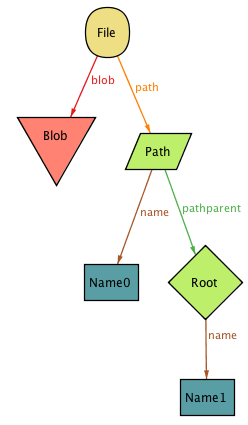
\includegraphics[scale=0.65]{images/image1.png}
\end{figure}
\pagebreak


\section{Index in Git}

The definition of Index:
"...staging area between your working directory and your
repository. You can use the index to {\bf build up a set of 
changes that you want to commit together}. When you create
a commit, {\bf what is committed is what is currently in the
index, not what is in your working directory.}"
\cite{gitComm} (page 17). \par

Also : ``The index {\bf contains all the information necessary to generate a single
(uniquely determined) tree object}'' \cite{gitComm} (pag 121). \par

Thus, what is in the index for a given state, is just a set of files.

\begin{lstlisting}
	sig File {
		path : Path,
		blob : Blob,
		index : set State
	}

\end{lstlisting}

\begin{figure}[h!] 
	\caption{A typical example of a file (file1) that is in the index}
	\centering
	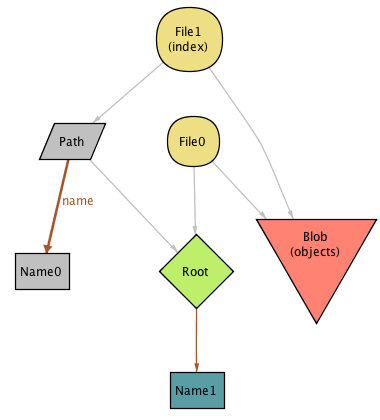
\includegraphics[scale=0.65]{images/image2.png}
\end{figure}
\pagebreak


\section {Modelling Git Dynamic Object Model}
The static object model, only by itself, 
is not very usefull. And so
the model would be much more interesting if we specify 
the most important git operations. That said in this
section we will focus on modelling the most important
and critical of them. \par

In order to understand them, the definition
of the git Working Directory and git Index is in debt.

\subsection{Introducing branches}
Definition of branch: "A branch in Git is {\bf simply a lightweight movable pointer to one of these commits}." \cite{progit} (pag 39)\\
A branch in git, is a pointer for a commit. We are always working on a certain branch, and all the commits made on that branch are independent from the others branch until we make a merge. A new branch can be created using \emph{git branch branch\_name}. The special pointer called Header points to the branch we are working on. We can go to another branch using \emph{git checkout branch\_name}.\\



Trying to understand branches using git:
\begin{itemize}
   \item if we modify a tracked file, we cannot change branch if we do not add that file to the index;
   \item if we add a tracked and modified file to the index and we change branch, that file will be presented as it was on the other branch;
   \item if we create a new file on a branch and then we change branch (without adding the file to the index) that file will be present;
   \item if we create a new file, add it to the index, change branch, commit, go back to the other branch, that file will not be visible;
   \item master branch can be deleted;
\end{itemize}

We can conclude that the index is not connected to a branch. It is something is common to all branches.
\subsection{Working Directory and Index}

The definition of Working Directory comes as follows:
"... simply a {\bf temporary checkout place} where you can 
modify the files {\bf until your next commit}."
\cite{gitComm} (pag 17). \par

To complement the definition above, git will only
track files that existed in the last commit, thus
new ones will not appear in this directory. \par 
So,
the Working Directory, does nothing more than telling
us wich files have been modified since the last commit.

\begin{lstlisting}
sig File{}
sig WorkingD {
	contents : set File
}
\end{lstlisting}

Now for the definition of Index:
"...staging area between your working directory and your
repository. You can use the index to {\bf build up a set of 
changes that you want to commit together}. When you create
a commit, {\bf what is committed is what is currently in the
index, not what is in your working directory.}"
\cite{gitComm} (page 17). So, the Index, in a certain
manner, points to a subset
of files that are present in the Working Directory, and
is this subset of files that wil be commited. 

\begin{lstlisting}
sig Index {
	toCommit : set File
}
\end{lstlisting}

However
there will be a few exceptions!(present in the last parapgrah of the sections
git add command and git rm command)\par

We can see  
that a commit depends on the contents of git Index, as the
last depends on the Working Directory. So it will be important
to add those definitions to our model when defining the commit operation
.But, a question arises.
What is the pratical difference between the Index and the Working
Directory? Shouldn't all that we modify in the repository be 
commited? We will see that next. 

\subsubsection{The git add command}

This command is one of the most used in git. \cite{gitComm} (page 26)
tells us that
"git add is {\bf used both for new and newly modified files},
and in both cases it takes a snapshot of the given files
and {\bf stages that content in the index, ready for inclusion
in the next commit}." \par 
When doing a git add of a newly
added file, that
addition will not appear in the Working Directory, only in the
Index. 
\subsubsection{The git rm command}

This one is generally less used. It's usefullness can be
seen in the following : \cite{progit}
(page 21) says "To remove a file from Git, you have to remove it
from your tracked files (more accurately, {\bf remove it from your
staging area}) and them commit. The {\bf git rm command does that
and also removes the file from your working directory}...". \par
Note that the working directory refered in the citation is not
the git Working Directory, it's the directory of the filesystem itself.
In other words a 'rm <file>' is present inside the 'git rm <file>'. \par
When using git rm
that modification will only appear in the Index. Unless, before
the git rm we delete the file from the filesystem (e.g. rm ). \par


\section{Conclusions}

\bibliographystyle{plain}
\bibliography{biblio}
\printglossary
\end{document}
